\documentclass[10pt, letterpaper]{report}
% !TeX program = xelatex
%==================PREAMBOLO=======================%
\usepackage[utf8]{inputenc}
\usepackage{psvectorian}
\usepackage{pgfplots}
\usepackage[Rejne]{fncychap}
\usepackage[export]{adjustbox}
\usepackage[T1]{fontenc}
\usepackage{lmodern}
\usepackage[shortlabels]{enumitem}
\usepackage{moresize}
\usepackage{graphicx} % Required for inserting images
\usepackage{hyperref}
\usepackage{listings}
\usepackage[table,xcdraw]{xcolor}
\usepackage{amssymb}
\usepackage{amsmath}
\usepackage[italian]{babel}
\usepackage{nicefrac, xfrac}
\usepackage{tikz}
\usepackage{mathrsfs} 
\usepackage{titletoc}
\usepackage{fancyhdr}
\usepackage{psvectorian,lipsum}
\usepackage{fourier-orns}
\usepackage{lipsum}
\usepackage[paper=a4paper,left=25mm,right=25mm,bottom=25mm,top=25mm]{geometry}
\definecolor{light-gray}{gray}{0.95}
\definecolor{cop}{HTML}{f7ecd7}
\definecolor{copAut}{HTML}{ababab}
\definecolor{copAut2}{HTML}{c3c3e6}
\definecolor{purcop}{HTML}{d0d3db}
\definecolor{sapienza}{HTML}{660f1d}
\definecolor{lightSapienza}{HTML}{e3d3d5}
\definecolor{darkgreen}{HTML}{008000}
\definecolor{cartaRiciclata}{HTML}{fcfcf7}
\newcommand{\redText}[1]{\color{red}#1\color{black}}
\newcommand{\code}[1]{\colorbox{light-gray}{\texttt{#1}}}
\newcommand{\codee}[1]{\colorbox{white}{\texttt{#1}}}
\newcommand{\K}{{\mathbb K}}
\newcommand{\notimplies}{%
  \mathrel{{\ooalign{\hidewidth$\not\phantom{=}$\hidewidth\cr$\implies$}}}}
\newcommand{\flowerLine}{ \begin{center}\decofourleft\hphantom{ }\decoone\hphantom{ }\decofourright\hphantom{}\hphantom{aa}
\decofourleft\hphantom{ }\decoone\hphantom{ }\decofourright\hphantom{}\hphantom{aa}
\decofourleft\hphantom{ }\decoone\hphantom{ }\decofourright\hphantom{}\hphantom{aa}
\decofourleft\hphantom{ }\decoone\hphantom{ }\decofourright\hphantom{}\hphantom{aa} 
\decofourleft\hphantom{ }\decoone\hphantom{ }\decofourright\hphantom{}\hphantom{aa}
\decofourleft\hphantom{ }\decoone\hphantom{ }\decofourright\hphantom{}\hphantom{aa}
\decofourleft\hphantom{ }\decoone\hphantom{ }\decofourright\hphantom{}\hphantom{aa}
\decofourleft\hphantom{ }\decoone\hphantom{ }\decofourright\hphantom{}\hphantom{aa}
\decofourleft\hphantom{ }\decoone\hphantom{ }\decofourright\hphantom{}\hphantom{aa}
\end{center}}
\definecolor{g}{RGB}{60, 50, 50}
\newcommand{\textg}[1]{\color{g}{\textbf{#1}}\color{black}}
\newcommand{\teo}[1]{{\large\color{sapienza}\textbf{Teorema #1 :\hphantom{a}}}}
\newcommand{\defi}[1]{{\large\color{sapienza}\textbf{Definizione #1 :\hphantom{a}}}}
\newcommand{\claim}[1]{{\color{sapienza}\textbf{Claim #1 :\hphantom{a}}}}
\newcommand{\lemma}[1]{{\color{sapienza}\textbf{Lemma #1 :\hphantom{a}}}}
\newcommand{\dimo}[1]{{\color{sapienza}\textbf{Dimostrazione #1 :\hphantom{a}}}}
\newcommand{\prop}[1]{{\color{sapienza}\textbf{Proposizione #1 :\hphantom{a}}}}
\newcommand\greybox[1]{%
  \vskip\baselineskip%
  \par\noindent\colorbox{light-gray}{%
    \begin{minipage}{\textwidth}#1\end{minipage}%
  }%
  \vskip\baselineskip%
}
\newcommand\sapbox[1]{%
  \vskip\baselineskip%
  \par\noindent\colorbox{lightSapienza}{%
    \begin{minipage}{\textwidth}#1\end{minipage}%
  }%
  \vskip\baselineskip%
}

\newcommand{\Z}{{\mathbb Z}}
\newcommand{\blank}{{\sqcup}}
\newcommand{\R}{{\mathbb R}}
\newcommand{\N}{{\mathbb N}}
\newcommand{\C}{{\mathbb C}}
\newcommand{\Sn}{{\mathcal S_n}}
\newcommand{\An}{{\mathcal A_n}}
\newcommand{\E}{{\mathcal E}}
\newcommand{\B}{{\mathcal B}}
\newcommand{\mcm}{{\text{mcm}}}
\newcommand{\rg}{{\text{rg}}}
\newcommand{\ve}{{\bar v}}
\newcommand{\spaz}{{\text{\hphantom{aa}}}}
\newcommand{\MCD}{{\text{MCD}}}
\newcommand{\tc}{{\text{ tale che }}}
\newcommand{\supp}{{\text{Supp}}}
\newcommand{\acc}{\\\hphantom{}\\}
\newcommand{\aut}{{\text{Aut}}}
\newcommand{\Span}{{\text{Span}}}
\newcommand{\End}{{\text{End}}}
\newcommand{\cen}{{\text{Centro}}}
\newcommand{\norm}{{\unlhd}}
\newcommand{\ciclS}{{\left \langle }}
\newcommand{\ciclE}{{\right \rangle }}
\newcommand{\boxedMath}[1]{\begin{tabular}{|c|}\hline \texttt{#1} \\ \hline\end{tabular} :}
\newcommand{\shell}[1]{\colorbox{black}{\textcolor{white}{\texttt{#1}}}}
\newcommand{\eqImportante}[1]{\begin{center}\huge\lefthand\hphantom{a}
    \normalsize\texttt{#1}
    \hphantom{aaa}\huge\righthand\end{center}}

\fancyhf{}
\pagestyle{fancy}
\usepackage{pgf-pie}  
\usetikzlibrary{positioning}

\renewcommand{\headrule}{%
\vspace{-8pt}\hrulefill
\raisebox{-2.1pt}{\quad\decothreeleft\decotwo\decothreeright\quad}\hrulefill}

%sta roba serve per il codice C
\definecolor{mGreen}{rgb}{0,0.6,0}
\definecolor{mGray}{rgb}{0.5,0.5,0.5}
\definecolor{mPurple}{rgb}{0.58,0,0.82}
\definecolor{backgroundColour}{rgb}{0.95,0.95,0.92}

\lstdefinestyle{CStyle}{
    backgroundcolor=\color{backgroundColour},   
    commentstyle=\color{mGreen},
    keywordstyle=\color{magenta},
    numberstyle=\tiny\color{mGray},
    stringstyle=\color{mPurple},
    basicstyle=\footnotesize,
    breakatwhitespace=false,         
    breaklines=true,                 
    captionpos=b,                    
    keepspaces=true,                 
    numbers=left,                    
    numbersep=5pt,                  
    showspaces=false,                
    showstringspaces=false,
    showtabs=false,                  
    tabsize=2,
    language=C
}
\lstdefinestyle{CppStyle}{
    backgroundcolor=\color{backgroundColour},   
    commentstyle=\color{mGreen}\ttfamily,
    morecomment=[l][\color{magenta}]{\#}
    keywordstyle=\color{blue}\ttfamily,
    numberstyle=\tiny\color{mGray},
    stringstyle=\color{red}\ttfamily,
    basicstyle=\ttfamily,
    breakatwhitespace=false,         
    breaklines=true,                 
    captionpos=b,                    
    keepspaces=true,                 
    numbers=left,                    
    numbersep=5pt,                  
    showspaces=false,                
    showstringspaces=false,
    showtabs=false,                  
    tabsize=2,
    language=C
}
\lstset{language=C++,
                basicstyle=\ttfamily,
                keywordstyle=\color{blue}\ttfamily,
                stringstyle=\color{red}\ttfamily,
                commentstyle=\color{green}\ttfamily,
                morecomment=[l][\color{magenta}]{\#}
}
%fine roba che serve per il codice C
\usepackage{minted}
 %TOGLI COMMENTO SE USI XELATEX
%\usepackage{fontspec}
\title{\jobname} %========TITOLO========%
\author{Marco Casu}
\date{\vspace{-5ex}}
\begin{document}

%==================COPERTINA=======================%
\begin{titlepage}
    \pagecolor{cartaRiciclata}
\begin{center}
    %TOGLI COMMENTO SE USI XELATEX
   %\setmainfont{Palace Script MT}
   \HUGE Marco Casu\acc
    %\setmainfont{Grand Casino}
     %TOGLI COMMENTO SE USI XELATEX
    %\setmainfont{h Halfroad}
    \HUGE \decothreeleft\hphantom{ }{\fontsize{48}{50}\selectfont \jobname}\hphantom{ }\decothreeright
     %TOGLI COMMENTO SE USI XELATEX
   % \setmainfont{Times New Roman}
\end{center}
\thispagestyle{empty}
\begin{figure}[h]
    \centering{
        %l'immagine deve avere una risoluzione 2048x2048
        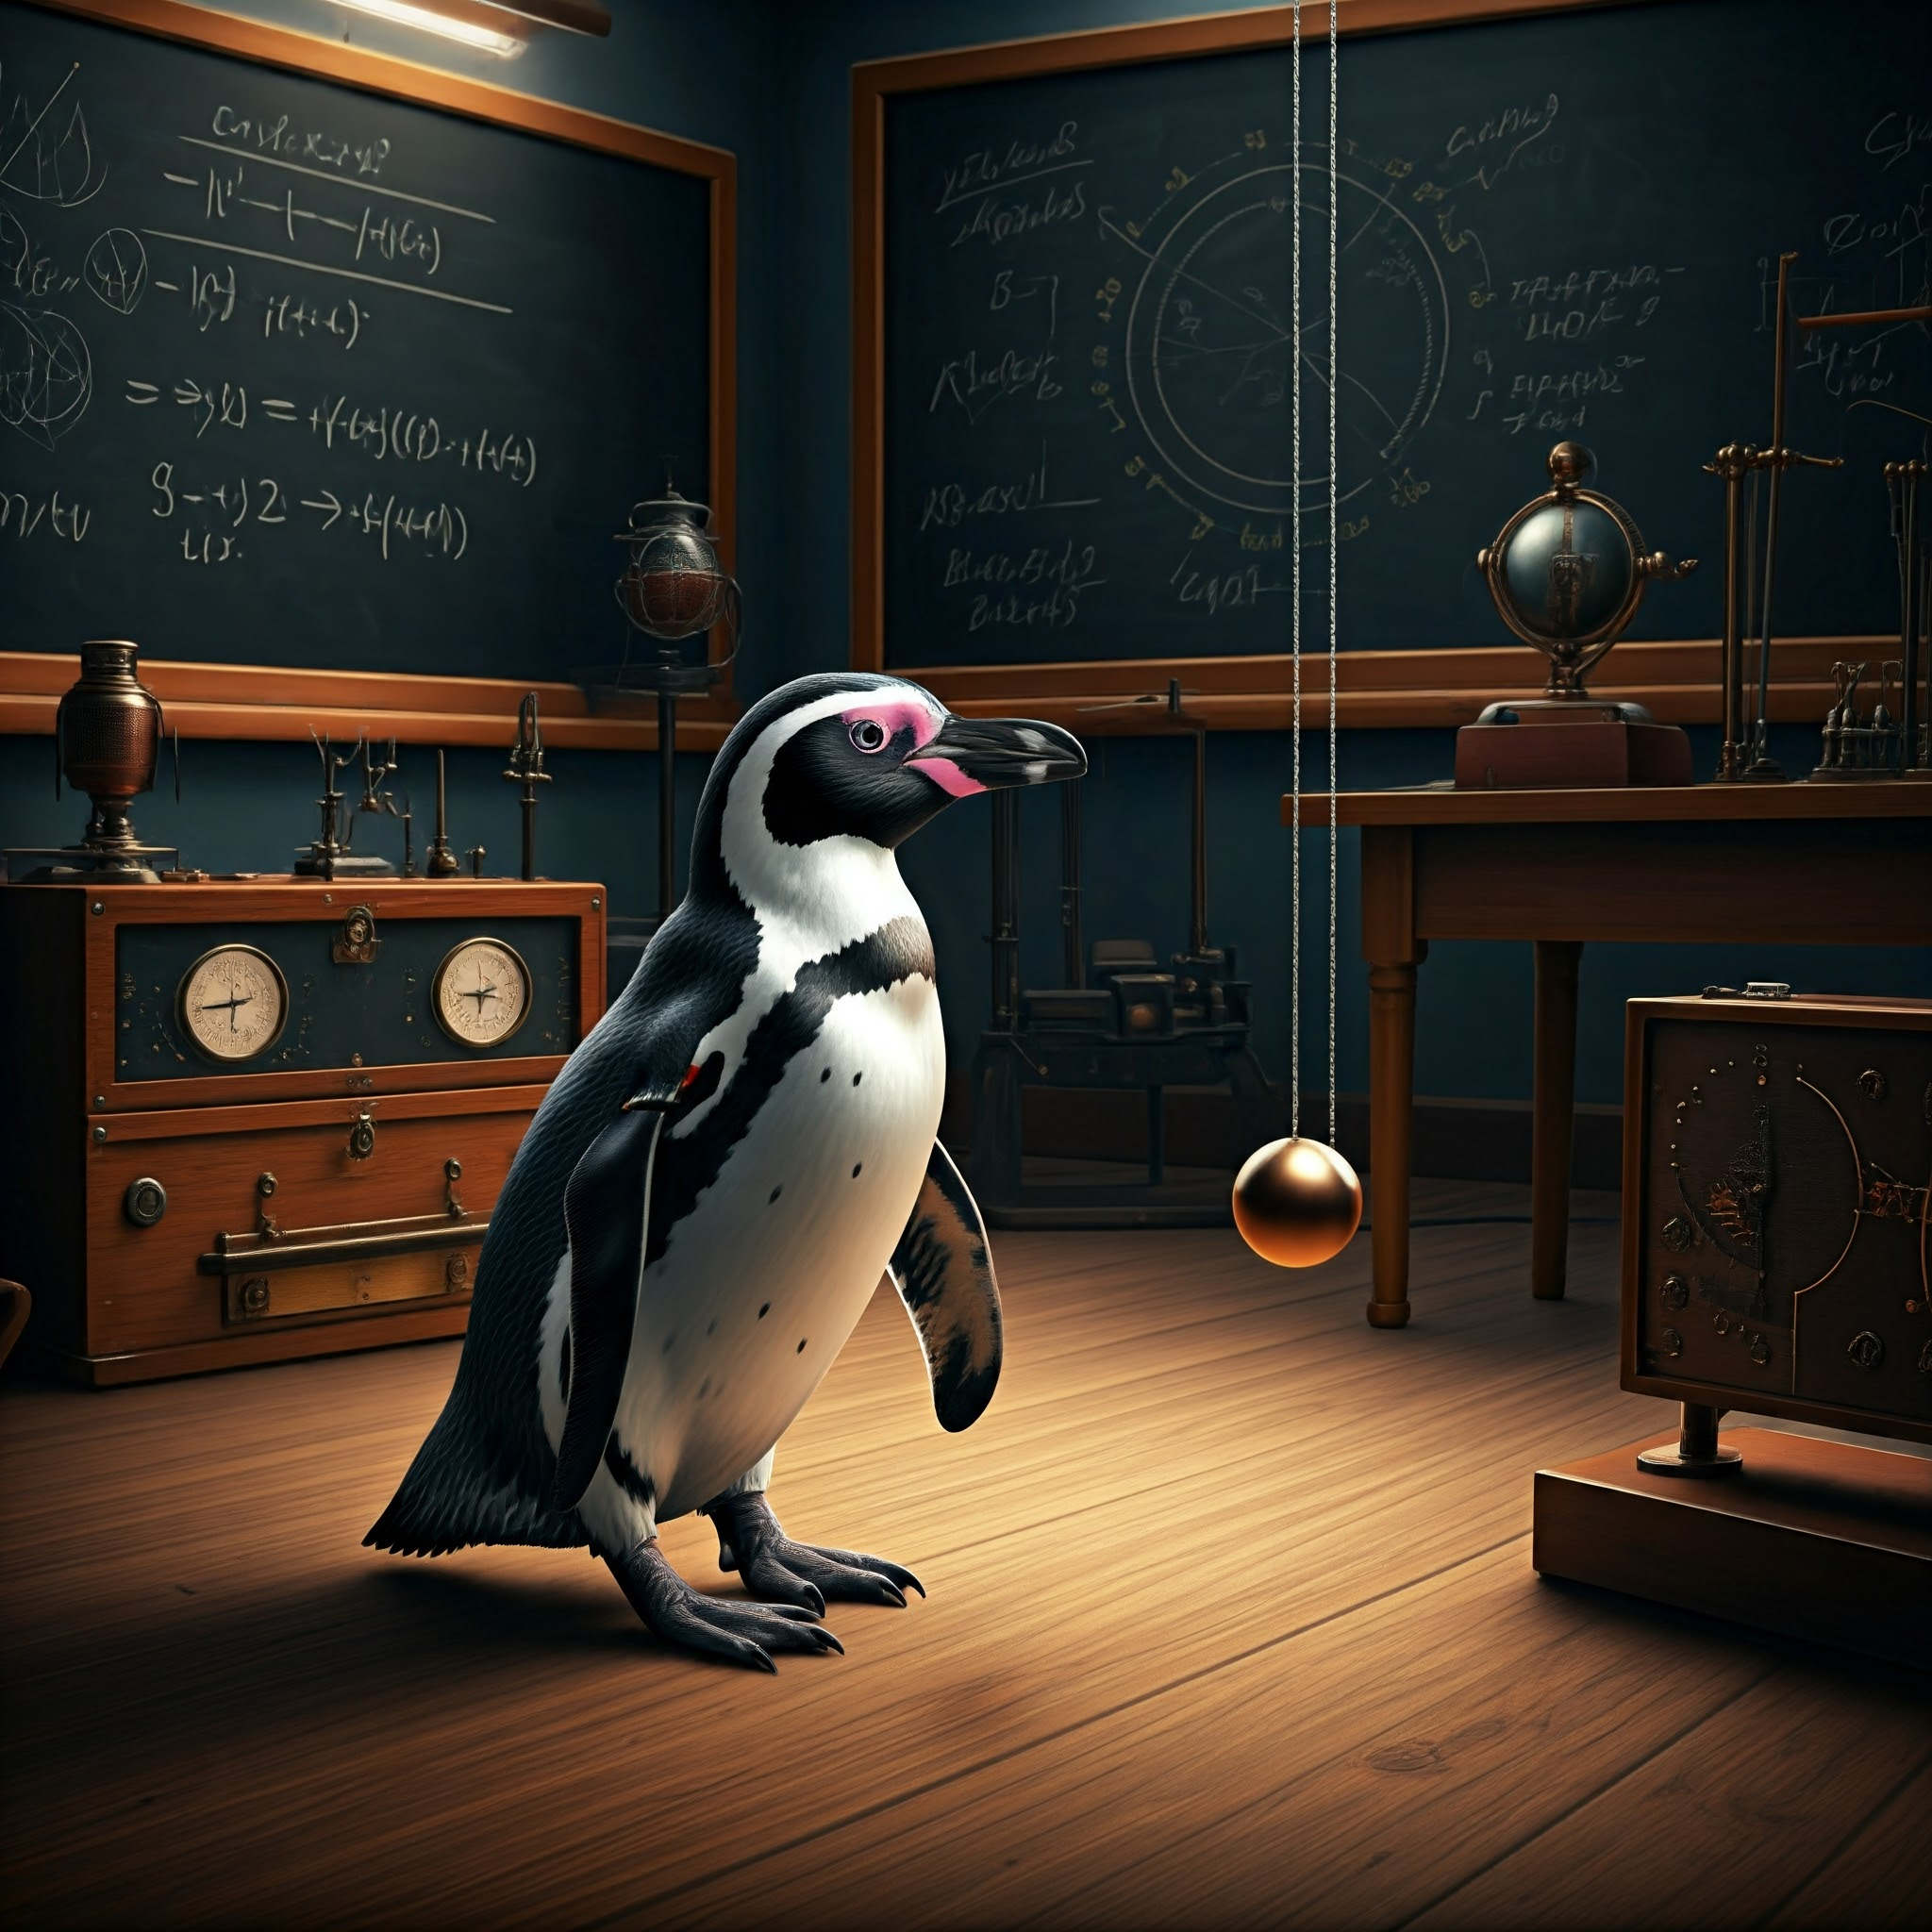
\includegraphics[width=1\textwidth ]{images/copertina.jpg}
    }
\end{figure}
\vfill 
\centering 
\includegraphics[width=0.4\textwidth ]{../../preamble/Stemma_sapienza.png} \acc
\centering \Large \color{sapienza}Facoltà di Ingegneria dell'Informazione,
Informatica e Statistica\\
Dipartimento di Informatica
\end{titlepage}

%===================FINE COPERTINA======================%
\newpage
\pagecolor{cartaRiciclata}%\setmainfont{Algerian}
Questo documento è distribuito sotto la licenza 
\color{blue}\href{https://www.gnu.org/licenses/fdl-1.3.txt}{GNU}\color{black},  
è un resoconto degli appunti (eventualmente integrati con libri di testo) tratti dalle lezioni del corso di \jobname
\hphantom{a}per la laurea 
triennale in Informatica. Se dovessi notare errori, ti prego di segnalarmeli.
\vfill
\begin{figure}[h!]
    \raggedright
    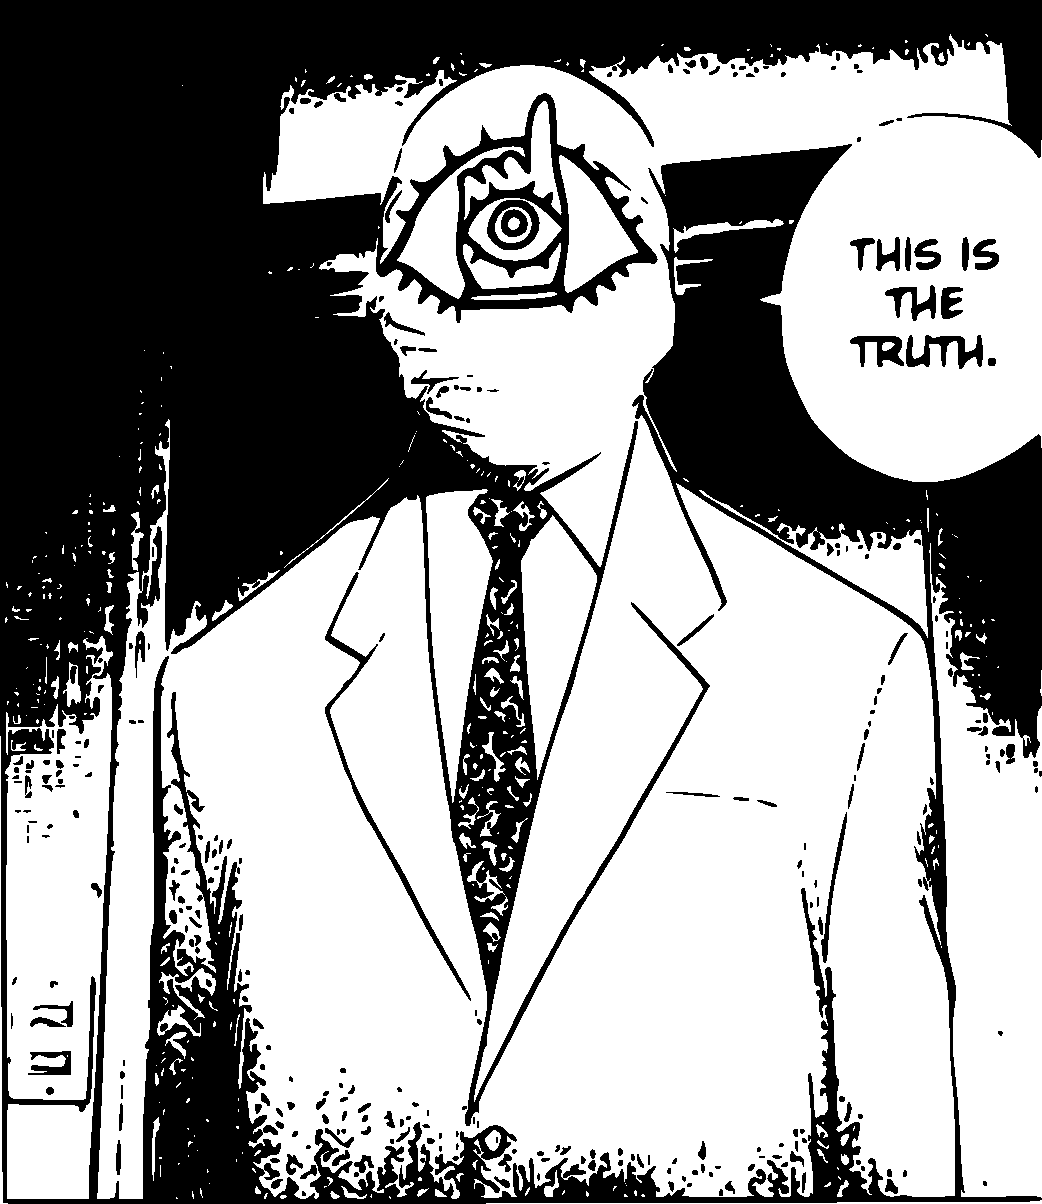
\includegraphics[width=0.4\textwidth,right ]{../../preamble/tomodachi.pdf} 
\end{figure}
\newpage %\setmainfont{Times New Roman}
\normalsize
\tableofcontents 
\newpage

%==================FOOTER e HEADER=======================%
\fancyhf{}
\fancyhead[L]{\nouppercase{\leftmark}}
\fancyhead[R]{Sezione \thesection}
\fancyfoot[C]{\thepage}
\fancyfoot[L]{Appunti di \jobname}
\fancyfoot[R]{ Marco Casu}
%\fancyfoot[R]{\setmainfont{Palace Script MT}\huge Marco Casu \setmainfont{Times New Roman}}
%==================FOOTER e HEADER=======================%

%Ricorda del comando \flowerLine per separare le sottosezioni. Le sezioni si separano nelle diverse pagine

%==================INIZIO======================%

\chapter{Introduzione}
\section{Il metodo scientifico}
La nascita del metodo scientifico è dovuta a Galileo Galilei, se i filosofi greci stabilivano 
leggi empiriche senza necessariamente dimostrarle, Galileo introdusse una verifica sperimentale 
a quelle che erano le sue digressioni.\acc 
Un \textbf{esperimento}, è una verifica sperimentale delle ipotesi, utile a ricavare valori 
numerici oggettivi per le misure delle grandezze fisiche. L'avvento del cannocchiale permise un 
osservazione più accurata dei corpi celesti, questi che venivano creduti perfetti, si rivelarono 
per quello che sono, la Luna con i suoi accavallamenti e "mari", mostrava una 
conformazione della sua crosta tutto fuorché perfetta.
\begin{figure}[h!]
    \centering
    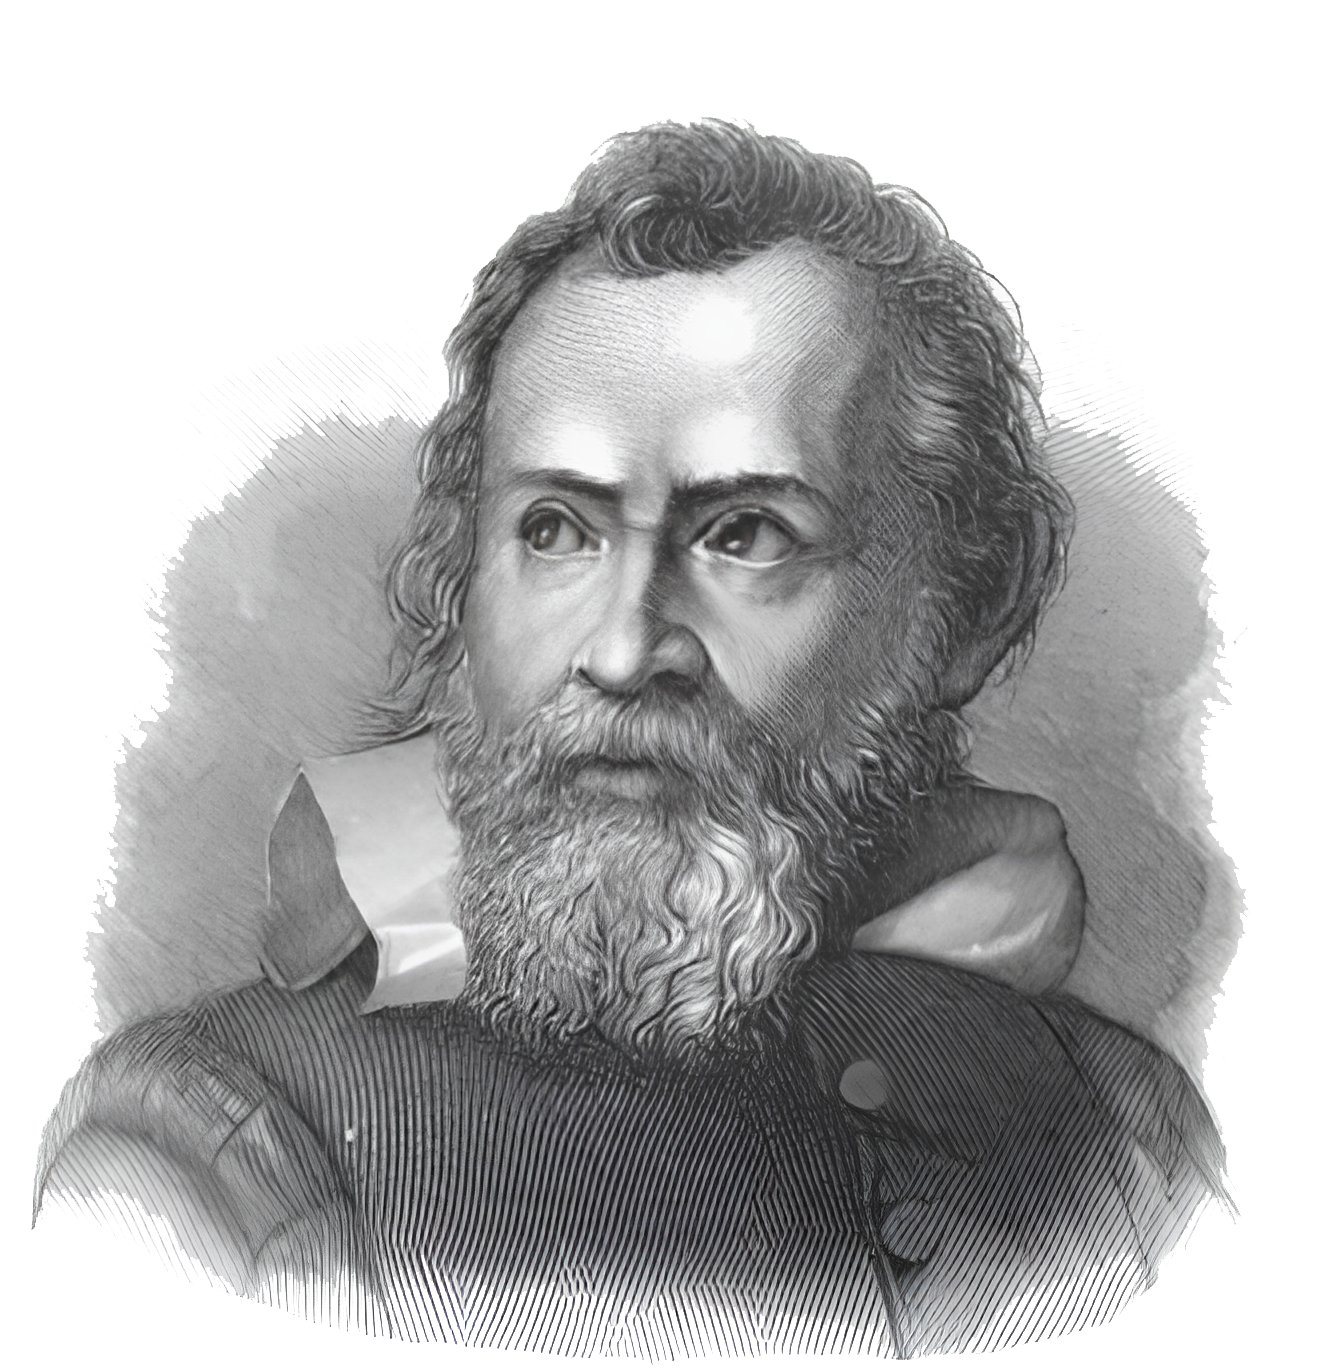
\includegraphics[width=140pt]{images/Galileo2.png}
    \caption{ Galileo Galilei}
    \label{fig:Galileo}
\end{figure}
Oltre al già citato cannocchiale, erano necessari ulteriori strumenti per le osservazioni dei 
corpi celesti, era necessario misurare in maniera precisa ed affidabile lo scorrere del tempo. 
Misurare il tempo vuol dire confrontare due eventi, ad esempio, il sorgere del sole con il movimento 
periodico riferito ad un misuratore (come l'orologio).\acc 
Galileo per le sue misure realizzò un orologio ad acqua, utilizzando un recipiente nella quale 
riporre un piccolo foro sul fondo, in modo tale che l'acqua cadesse a gocce a velocità costante, 
così facendo, lo scorrere del tempo era proporzionale al volume dell'acqua perso dall recipiente.\acc 
Una \textbf{grandezza fisica} è un entità alla quale si attribuisce una specifica definizione, utilizzabile 
per descrivere un fenomeno fisico, per tali entità devono valere i criteri di uguaglianza e 
sommabilità.\acc 
Uno degli argomenti su cui si soffermò Galileo fu il \textit{moto dei gravi}, in particolare 
il moto dei corpi in caduta libera. Secondo la fisica aristotelica del tempo, un corpo 
tanto più pesante era, tanto più rapidamente cadeva. \acc 
Galileo fu critico nei riguardi di questa visione, osservò che in realtà, ogni corpo 
cade verso il suolo con la stessa accelerazione, il motivo per il quale una piuma cade 
più rapidamente di una sfera di piombo non riguarda la loro massa, bensì la resistenza dell'aria 
nei confronti del loro materiale e della loro forma. Trovò inoltre che la distanza percorsa 
durante la caduta di un oggetto è proporzionale al quadrato del tempo impiegato per percorrerla.\acc 
Galileo con un esperimento riguardante i piani osservò il seguente fatto : 
    \textit{se si lascia scivolare un corpo su un piano inclinato ad altezza $h$ per poi 
    farlo risalire su un altro piano inclinato, questo tendeva a risalire fino alla 
    stessa altezza $h$}.
    \begin{figure}[h!]
        \centering
        \includegraphics[width=500pt]{images/cadutaGraveBW.eps}
        \caption{ caduta sul piano inclinato}
        \label{fig:caduta}
    \end{figure}\acc
Inoltre, notò che questo fenomeno non è condizionato dal seno dell'angolo del piano, bensì 
esclusivamente dall'altezza.
\begin{figure}[h!]
    \centering
    \includegraphics[width=500pt]{images/cadutaGrave2BW.eps}
    \caption{ inclinazioni differenti}
    \label{fig:caduta2}
\end{figure}\acc
Per osservare tale risultato dovette ridurre le azioni spurie dell'attrito dell'aria. Più 
il percorso era liscio, più l'attrito risultava debole, e più il corpo tendeva ad 
avvicinarsi all'altezza originale $h$. Con tale ragionamento ipotizzò che se l'attrito dovesse 
essere stato nullo, allora il corpo sarebbe tornato precisamente all'altezza $h$.\acc 
Dato questo per vero, riducendo il valore dell'angolo sarebbe stato possibile far percorrere 
al corpo una distanza maggiore. Se il secondo piano avesse avuto inclinazione nulla, allora 
il grave avrebbe continuato a muoversi in avanti a velocità costante.\begin{figure}[h!]
    \centering
    \includegraphics[width=330pt]{images/cadutaGrave3BW.eps}
    \caption{ inclinazione nulla}
    \label{fig:caduta3}
\end{figure}\acc
Tale principio è noto come \textbf{legge d'Inerzia}, eliminando gli attriti, lo stato di moto naturale inalterato di
un corpo è quello di moto rettilineo uniforme (a velocità costante) indefinitamente.\acc 
Essendo la scienza sempre stata impiegata anche in ambito bellico, Galileo studiò il moto dei 
proiettili, che fino a quel momento si credeva fosse costantemente orizzontale, fino al momento in 
cui il proiettile perdeva il suo "impeto" cadendo a terra. Egli si rese conto che 
i proiettili sono soggetti sia alla forza impressa dal colpo (orizzontale), sia a quella verticale 
impressa verso il basso.\acc 
La forza impressa dal colpo gli da una velocità costante, in quanto non è soggetto ad ulteriori 
accelerazioni orizzontalmente, quella verticale invece provoca un moto uniformemente accelerato, 
la distanza 
percorsa in verticale è proporzionale al 
quadrato del tempo impiegato a percorrerla, la combinazione dei due moti risulta in un arco 
di parabola.
\begin{center}
	\begin{tabular}{>{\centering\arraybackslash}m{3in}>{\centering\arraybackslash}m{3in}}
		\begin{tikzpicture}[scale=0.9, transform shape]
		\begin{axis}[
		ymin=-6,
		ymax = 6,
		xmin=-6,
		xmax = 6,
		axis lines = center,
		xtick distance=2, ytick distance=2,
		grid style=dashed,
		ymajorgrids=true,
		xmajorgrids=true,
		xlabel = \(\),
		ylabel = {\(\)},
		]
		%Below the red parabola is defined
		\addplot [
		domain=-6:6,
		samples=20,
		color=blue,
		]
		{-(1/5)*(x^2)};
		\addlegendentry{\(y=-\nicefrac{1}{5}\cdot x^2\)}
		\end{axis}
		\end{tikzpicture} &   
		Galileo, chiamò $x$ la direzione orizzontale, ed $y$ quella verticale, partendo da 
		$(x,y)=(0,0)$, e sapendo che lo spazio percorso in $x$ è proporzionale ale tempo, mentre 
		quello percorso in $y$ è proporzionale al quadrato del tempo, si ha 
		$$ x=a\cdot t\;\;\;\;\;\;\;\;\;\;\;\; y = b\cdot t^2$$
		Con alcuni passaggi algebrici si trova esattamente la nota equazione della parabola
		$$ y=\frac{b}{a^2}\cdot x^2$$
		\\
	\end{tabular}
\end{center}
\flowerLine 
\section{Spostamento, Velocità e Grandezze Fisiche}
Il \textbf{moto}, è uno dei fenomeni fisici più classici, che necessita 
di una definizione e rappresentazione formale, è il cambiamento 
di una posizione rispetto al tempo.\acc 
Un classico esempio di sistema di riferimento è il piano cartesiano, 
in cui un punto nello spazio, è identificato da tre coordinate 
$$ (x(t),y(t),z(t))$$
In funzione del tempo $t$. Può essere rappresentato anche da 
un vettore posizione $\bar r(t)$, descritto dalla lunghezza 
e dagli angoli rispetto gli assi del piano e la proiezione 
delle sue componenti, nel caso bi-dimensionale, sia $r$ il modulo 
del vettore $\bar r$ :
\begin{figure}[h!]
    \centering
    \includegraphics[width=100pt]{images/vecAngolo.eps}
    \caption{ $\bar r = (r,\theta)$}
    \label{fig:vecAng}
\end{figure}\acc 
Risulta possibile passare dalle coordinate cartesiane a quelle descritte 
con l'angolo tramite le seguenti trasformazioni 
$$\begin{cases}
    r\cos(\theta)=x\\ r\sin(\theta)=y
\end{cases} $$
Inoltre 
$$r^2(\cos^2(\theta)+\sin^2(\theta))=x^2+y^2$$
$$r=\sqrt{x^2+y^2}\ \ \ \ \ \ \ \ \theta = \arctan(\nicefrac{y}{x})$$
Le componenti di $\bar r$ dipendono dal sistema di riferimento.
Posso definire uno \textit{spostamento nel tempo}, tramite il vettore 
$\bar r$ in un istante $t$, ed il medesimo vettore in un istante 
$t+\Delta t$, dove $\Delta t$ rappresenta una variazione temporale. 
Una volta definiti i vettori $\bar r (t)$ e $\bar r (t+\Delta t)$,
 si definisce il \textbf{vettore spostamento} come la loro 
 differenza algebrica, ossia $\Delta \bar r = \bar r (t+\Delta t)-\bar r (t)$.
 \begin{center}
    \centering
    \begin{minipage}{.5\textwidth}
      \centering
      \includegraphics[width=.5\linewidth]{images/spostamento.eps}
    \end{minipage}%
    \begin{minipage}{.5\textwidth}
      \centering
      \includegraphics[width=.5\linewidth]{images/vecSpostamento.eps}
    \end{minipage}
\end{center}
Si vogliono rappresentare i vettori in maniera più formale, rispetto 
che alla classica notazione $\bar v = (x,y,z)$. Si fa uso dei versori 
$$ \bar i = (1,0,0)\ \ \ \
\bar j = (0,1,0)\ \ \ \  
\bar k = (0,0,1) $$
per definire un vettore come somma dei versori scalati con appositi 
 coefficienti, che rappresentano le componenti del vettore : 
 $$ \bar v = (x,y,z) = x\bar i+y\bar j+z \bar k $$
 Ogni componente della somma è la proiezione del vettore su uno dei 
 tre assi. Si osservi come il vettore spostamente non dipende dal sistema di riferimento.\acc 
 Il vettore spostamento $\Delta \bar r$ varia a sua volta nel tempo, 
 descrivendo quindi il moto di un punto, la \textbf{velocità media} di tale 
 spostamento si definisce tramite il rapporto incrementale 
 $$ 
 \frac{\Delta \bar r (t)}{\Delta t}=\frac{\bar r(t+\Delta t)-\bar r(t)}{\Delta t}
 $$
Si può definire anche la velocità media scalare, se lo spostamento avviene 
su un percorso già definito, e non è necessaria informazione sulla 
direzione, è possibile rappresentarlo con uno scalare 
$s(t)$, e $\dfrac{\Delta s}{\Delta t}$ rappresenta la velocità media 
scalare.\acc 
La velocità media non è molto precisa come informazione, in quanto 
non descrive il moto di un corpo (la sua traiettoria) a pieno, 
si vuole quindi dare una misura di una velocità \textit{istantanea}, 
si fa quindi tendere a zero la differenza di tempo : 
$$
\lim_{\Delta t\rightarrow 0} \frac{\Delta \bar r (t)}{\Delta t}=
\lim_{\Delta t\rightarrow 0} \frac{\bar r(t+\Delta t)-\bar r(t)}{\Delta t}
$$
Tale grandezza si denota $\dfrac{d\bar r}{d t}$, è la derivata 
dello spostamento rispetto al tempo, verrà nominata semplicemente  
\textbf{velocità}, e denotata $\bar v$,  rappresenta lo spostamento istantaneo ed è 
tangente alla curva dello spostamento. Si definisce anche la 
velocità scalare  $\dfrac{d s}{d t}$, ed è il modulo della 
velocità.\acc 
Una volta definite delle quantità come spostamento e velocità, è necessario 
definire delle \textit{grandezze fisiche} ed introdurre delle 
\textit{unità di misura}. Il vettore $\bar r$ ha le dimensioni di una lunghezza, la dimensione 
lunghezza $[l]$ è espressa in metri $m$, il sistema internazionale definisce  
$$ (m,kg,s)=\text{ (metri, kilogrammi, secondi)}$$
La dimensione del tempo $[t]$ è espressa in secondi $s$. Esistono alcune grandezze 
dette adimensionali, un esempio sono gli angoli, misurati in gradi o radianti.
\acc 
La velocità, è una grandezza derivata, essendo un rapporto fra lo spostamento ed il tempo, 
si misura in metri al secondo : $\nicefrac{m}{s}$, rappresenta, appunto la distanza in 
metri percorsa in 1 secondo. Le grandezze possono essere convertite, ad esempio, considerando 
i kilometri - orari si ha che 
$$ 1\nicefrac{m}{s}= 
\frac{10^{-3}}{\nicefrac{1}{3600}}\nicefrac{km}{h}= 
10^{-3}\cdot 3600 \nicefrac{km}{h}=3.6\nicefrac{km}{h}$$
Introduciamo adesso il concetto di \textbf{differenziale}, si consideri una generica funzione 
$f(x)$ in un punto $x_0$, ed il suo rapporto incrementale per una variazione $d x$.
\begin{center}
	\begin{tabular}{>{\centering\arraybackslash}m{3in}>{\centering\arraybackslash}m{3in}}
		\includegraphics[width=.8\linewidth]{images/differenziale1.eps} & Il segmento denotato \color{blue}$\Delta f(x)$ \color{black} rappresenta l'incremento 
        effettivo della funzione, e vale $f(x_0+d x)-f(x_0)$.
		\\
	\end{tabular}
\end{center}
Definisco ora il \textbf{differenziale} 
di $f$ come una  \textbf{linearizzazione} della funzione, ossia, si considera nel punto $x_0$ una 
retta tangente alla curva di $f$.
\begin{center}
	\begin{tabular}{>{\centering\arraybackslash}m{3in}>{\centering\arraybackslash}m{3in}}
		\includegraphics[width=.8\linewidth]{images/differenziale2.eps} &Il differenziale \color{darkgreen} $df$ \color{black}da una stima dell'incremento, considerando una funzione lineare (in questo 
        caso bidimensionale, una retta).
		\\
	\end{tabular}
\end{center}
Denotando con $f'$ la derivata di $f$ si ha
$$ df=f'\cdot dx$$
$$ \frac{df}{dx}=f'$$
Le funzioni lineari sono più semplici di quelle non lineari, il punto di tale differenziale 
è che, quando l'incremento $d x$ tende a zero, l'incremento effettivo della funzione 
e l'incremento "stimato" dato dal differenziale tendono allo stesso valore. $$ 
\lim_{d x\rightarrow 0 }f(x_0+dx)=f(x_0)+f'(x_0)\cdot dx
$$
\chapter{Cinematica}
Si è introdotto il vettore spostamento $\delta \bar r$, con la sua relativa formulazione infinitesima 
di velocità $\bar v$, come derivata del vettore posizione $\bar r$. 
Un'altra grandezza fondamentale nello studio del moto dei corpi è la variazione della velocità, definita 
come il limite del rapporto incrementale di quest'ultima rispetto al tempo. 
Tale grandezza prende il nome di \textbf{accelerazione}
$$ \frac{d\bar v}{d t} = \bar a $$
L'accelerazione $\bar a$, o $a$ se riferita ad una grandezza scalare, si misura in 
$\nicefrac{m}{s^2}$, di cui l'unità, indica che ad ogni secondo, la velocità aumenta 
di $1 \nicefrac{m}{s}$, ovviamente anche'essa può dipendere dal tempo. 
$$\bar a=\frac{d\bar v}{dt}=\frac{d^2\bar r}{dt^2}$$
Si consideri adesso lo spostamento in forma scalare $s(t)$, definito su una traiettoria 
curvilinea già definita
\begin{center}
    \begin{figure}[h!]
        \centering
        \includegraphics[width=0.4\textwidth]{images/accScal.eps}
        \caption{velocità scalare}
        \label{fig:velScal}
    \end{figure} 
\end{center}
Di quest'ultima ne voglio ricavare la sua versione vettoriale, sia $\bar\tau(t)$ il versore 
tangente alla curva prestabilita, nell'immagine \ref{fig:velScal}, evidenziato in blu. 
Si avrà che la velocità vettoriale sarà 
$$ \bar v(t)=\dot{s}(t)\cdot \bar\tau(t)$$
Appunto sulla notazione :  $\dot{s}$ è la derivata prima di $s$. 
$\ddot{s}$ è la derivata seconda di $s$. A questo punto è possibile riscrivere 
l'accelerazione nella seguente forma :
$$
\bar a = \dfrac{d}{dt}\bar v(t)=\ddot{s}(t)\cdot \bar\tau(t)+\dot{s}(t)\cdot\dot{\bar\tau}(t)
$$
Si è quindi divisa l'accelerazione in due componenti distinte, la componente 
$\ddot{s}(t)\cdot \bar\tau(t)$ è nota come \textbf{accelerazione tangenziale} e rappresenta 
la variazione nel tempo del modulo della velocità. L'altra componente, verrà ripresa in seguito, 
ha a che fare con la curvatura della traiettoria.\acc 
\section{I Moti}
\subsection{Rettilineo Uniforme} 
Il moto rettilineo uniforme, secondo la legge d'Inerzia, descrive il moto naturale degli 
oggetti quando non sono soggetti a forze. Tale moto è contraddistinto dal fatto che 
l'accelerazione sia nulla, e la velocità costante, (per semplicità, verranno trattate 
le grandezze in forma scalare).
$$\frac{dv}{dt}=0\implies v = v_0 \text{ costante }$$
Si può ricavare facilmente l'equazione dello spostamento $r$ in un 
lasso di tempo che va da $t_0$ fissato, ad un $t$ generico
$$ \frac{dr}{dt}=v=v_0\implies dr=vd_0t\implies\int_{r(t_0)}^{r(t)}dr=\int_{t_0}^tv_0dt $$
$$\int_{t_0}^tv_0dt=v_0\int_{t_0}^tdt=v_0(t-t_0) $$
Si ha che  
$$ r(t)=r(t_0)+v_0(t-t_0)$$
L'equazione che descrive il moto rettilineo uniforme è lineare
\begin{center}
    \begin{tikzpicture}[scale=0.6, transform shape]
        \begin{axis}[
        ymin=0,
        ymax = 3,
        xmin=0,
        xmax = 3,
        axis lines = left,
        xtick distance=0.5, ytick distance=0.5,
        grid style=dashed,
        ymajorgrids=true,
        xmajorgrids=true,
        xlabel = \(t\),
        ylabel = {\(r(t)\)},
        ]
        %Below the red parabola is defined
        \addplot [
        domain=0:3,
        samples=20,
        color=blue,
        ]
        {x};
        \end{axis}
    \end{tikzpicture}
\end{center} 
\subsection{Uniformemente Accelerato}
La caratteristica del moto uniformemente accelerato è quella di avere un accelerazione costante 
$a = a_0 $, si avrà che 
$$ \frac{dv}{dt}=a_0\implies dv =a_0dt\implies \int_{v(t_0)}^{v(t)}dv=\int_{t_0}^tadt\implies$$
$$v(t)=v(t_0)+a_0(t-t_0) $$
Per semplicità, si definisce $v_0=v(t_0)$ la velocità iniziale. A questo punto, avendo nota l'equazione 
della velocità, si ricava la legge oraria, sia $x_0=x(x)$ la posizione iniziale 
$$ \frac{dx}{dt}=v\implies \int_{x_0}^{x(t)}dx=\int_{t_0}^t vdt = \int_{t_0}^tv_0+a_0(t-t_0)dt= 
v_0\int_{t_0}^tdt+a_0\int_{t_0}^t(t-t_0)dt$$
Considero $t'=t-t_0\implies dt'=dt$ 
$$ v_0\int_{t_0}^tdt+a_0\int_{t_0}^t(t-t_0)dt= 
v_0\int_{t_0}^tdt+a_0\int_{0}^{t-t_0}t'dt'=v_0(t-t_0)+\Big[\dfrac{1}{2}a_0t'\Big]_0^{t-t_0}$$
La soluzione oraria è quindi 
$$ x(t)=x_0+v_0\cdot (t-t_0)+\frac{1}{2}a_0\cdot (t-t_0)^2$$
Essa risulta essere l'equazione della parabola, nel caso più semplice in cui la posizione 
iniziale è 0, ed il tempo iniziale pure, si ha  
$$ x(t)=\dfrac{1}{2}a_0t$$
lo spazio percorso è proporzionale al tempo al 
quadrato.
\subsection{Caduta dei Gravi}
La caduta degli oggetti verso il suolo è descritta dal moto uniformemente 
        accelerato. Ogni oggetto nel campo gravitazionale terrestre, all'altezza del mare, subisce un 
        accelerazione di gravità pari a 
        $$ g\simeq 9.81 \nicefrac{m}{s^2}$$ 
        diretta verso il centro della terra. 
\begin{center}
	\begin{tabular}{>{\centering\arraybackslash}m{3in}>{\centering\arraybackslash}m{3in}}
        \includegraphics[width=0.35\textwidth]{images/oggettoLasciatoCadere.eps} & Definiamo un sistema di riferimento in cui il suolo 
        rappresenta lo zero, ed un corpo viene lasciato cadere da un altezza $h$. Per semplicità, 
        il tempo iniziale $t_0$ è uguale a $0$.
		\\
	\end{tabular}
\end{center}
La legge orario che descrive la posizione $y$ dell'oggetto è la segunete 
$$ \begin{cases}
    y(t)=h-\frac{1}{2}gt^2 \\ 
    v(t)=\dfrac{dy}{dt}=-gt
\end{cases}$$
È possibile calcolare l'istante $t^*$ in cui l'oggetto toccherà il suolo : 
\begin{eqnarray} y(t^*)=0\implies h-\frac{1}{2}g{t^*}^2 =0 \\ 
     h=\frac{1}{2}g{t^*}^2 \\ 
     2\frac{h}{g}={t^*}^2 \\ 
     t^*=\sqrt{2\frac{h}{g}}
\end{eqnarray}
\begin{center}
	\begin{tabular}{>{\centering\arraybackslash}m{3in}>{\centering\arraybackslash}m{3in}}
        \includegraphics[width=0.35\textwidth]{images/graveCaduta2.eps} & Se l'oggetto venisse inizialmente lanciato verso l'alto, si avrebbe una velocità iniziale 
        $v_0$ diversa da zero. La forza di gravità agirà sulla velocità dell'oggetto, facendola diminuire fino a farla 
        diventare negativa, facendolo ricadere verso il suolo.
		\\
	\end{tabular}
\end{center}
L'equazione oraria sarebbe$$ \begin{cases}
    y(t)=h+v_0t-\frac{1}{2}gt^2 \\ 
    v(t)=\dfrac{dy}{dt}=v_0-gt
\end{cases}$$
È possibile trovare il punto più alto raggiunto dal grave, esso sarà il punto in cui la velocità 
passerà da essere positiva (l'oggetto si allontana dal suolo) ad essere negativa (l'oggetto si avvicina al suolo), 
raggiungerà quindi il punto più alto nell'istante $t^*$ in cui la velocità è nulla. 
$$ v(t^*)=0\implies v_0-gt^* = 0 \implies t^*=\frac{v_0}{g}$$
La quota massima raggiunta sarà quindi 
\begin{eqnarray}
    t(\nicefrac{v_0}{g}) = h+v_0\nicefrac{v_0}{g}-\frac{1}{2}g(\nicefrac{v_0}{g})^2 =\\ 
    h+\frac{v_0^2}{g}-\frac{v_0}{2g} = \\ 
    h+\frac{1}{2}\frac{v_0^2}{g}
\end{eqnarray}
È possibile riscrivere l'equazione del moto uniformemente accelerato in funzione dello 
\textit{spazio percorso} partendo da un punto $x_0$ 
$$ \begin{cases}
    x=x_0+v_0t+\frac{1}{2}at^2\\ 
    v=v_0+at
\end{cases}\implies x-x_0=v_0t+\frac{1}{2}(v-v_0)t \implies x-x_0=\frac{1}{2}(v_0+v)t$$
\subsection{Moto del Proiettile}
Si vuole modellizzare la traiettoria di un proiettile, sparato con una certa angolazione, si 
considera quindi il piano cartesiano $(x,y)$, e la legge oraria sarà descritta da un 
vettore $\bar r(t)=(x(t),y(t))$ che ne descrive lo spostamento sui due assi.\acc 
Il proiettile è soggetto a due forze, la prima è la velocità orizzontale, data al tempo 
$t_0$ dallo sparo, la seconda è l'accelerazione di gravità, che gli conferisce una velocità 
verticale uniformemente accelerata. Denotiamo $v_x$ e $v_y$ le due velocità, $(x_0,y_0)$ la 
posizione iniziale, e $({v_y}_0,{v_x}_0)$ la velocità iniziale. Per semplicità, l'istante di inizio 
sarà $0$.
$$\begin{cases}
    y(t)=y_0+{v_y}_0t-\frac{1}{2}gt^2\\ 
    v_y(t)=v_{y_0}-gt
\end{cases} \text{ verticalmente}$$
$$ x(t)=x_0+v_{x_0}t\text{ orizzontalmente}$$
\begin{center}
    \begin{figure}[h!]
        \centering
        \includegraphics[width=0.6\textwidth]{images/motoProiettile.eps}
        \caption{moto del proiettile}
        \label{fig:pro}
    \end{figure} 
\end{center}
L'altezza massima si ha nell'istante $t^*$ in cui $v_y(t^*)=0\implies t^*=\frac{v_{y_0}}{g}$.
Con il termine \textit{gittata}, si intende la distanza $R$ percorsa dal proiettile orizzontalmente, 
essa è uguale a $R=v_{x_0}\cdot t_{tot}$, dove $t_{tot}$ è l'istante in cui il proiettile raggiunge 
il suolo, terminando la traiettoria e vale $t_{tot}=2\frac{v_{y_0}}{g}$.
$$ R=v_{x_0}\cdot2\frac{v_{y_0}}{g}$$ La velocità totale iniziale del proiettile, risulta 
essere 
$$ v_0=\sqrt{v_{x_0}^2+v_{x_y}^2}$$
Si può esprimere la gittata in funzione dell'angolo $\theta$ in cui si lancia il proiettile rispetto 
l'asse delle ascisse 
$$ R(\theta)=\frac{2v_0^2\sin(\theta)\cos(\theta)}{g}$$
A tal punto, si vuole esprimere l'angolo $\theta$ che massimizza la gittata. Essendo che $R(\theta)$ descrive 
la variazione della gittata al variare di $\theta$, è necessario trovare l'angolo in cui la derivata 
di $R$ si annulla, si considera 
$$ \frac{dR}{d\theta}=\frac{2v_0^2}{g}(\cos^2(\theta)-\sin^2(\theta))$$
Si pone a zero e si risolve per $\theta$
\begin{eqnarray}
    \frac{2v_0^2}{g}(\cos^2(\theta)-\sin^2(\theta))=0 \implies\\ 
    (\cos^2(\theta)-\sin^2(\theta))=0\implies\\ 
    \cos^2(\theta)=\sin^2(\theta)\implies \\ 
    \theta = \frac{\pi}{4}=45^\circ
\end{eqnarray}
\subsection{Moto Circolare Uniforme}
Si vuole descrivere il moto di un corpo, che rotea attorno ad un centro il cui modulo della 
velocità è costante. È importante specificare che il modulo sia costante, in quanto la velocità 
costante indica una non-variazione della direzione, invece nel moto circolare, la direzione 
cambia nel tempo, quindi vi sarà un accelerazione non nulla.\begin{center}
    \begin{figure}[h!]
        \centering
        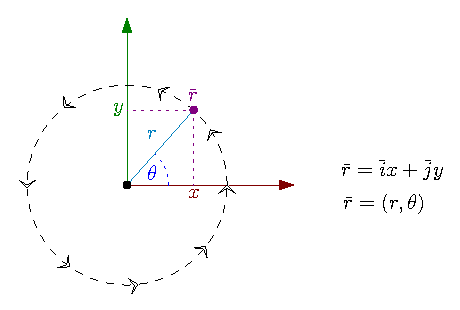
\includegraphics[width=0.5\textwidth]{images/motoCircUn.eps}
    \end{figure} 
\end{center}
Sia $\bar v$ la velocità, essendo il modulo costante, denoteremo $|\bar v|=v_0$. Si considera ora 
la velocità scalare $s$, di cui si ricorda 
$$ \frac{ds}{dt}=v_0$$
Inoltre, sapendo che $\frac{s}{R}=\theta$, si pone 
$$ \frac{ds}{R}=d\theta \implies \frac{ds}{dt}=R\cdot \frac{d\theta}{dt}=v_0$$
Denotiamo $\omega = \dfrac{d\theta}{dt}$, tale termine descrive la variazione dell'angolo nel tempo 
ed è denominato \textbf{velocità angolare}. Il fatto che la velocità dipenda dal raggio $R$, descrive il fatto 
che a parità di velocità angolare, un oggetto che si muove su un cerchio di raggio minore va meno veloce. 
$$ \frac{d\theta}{dt}=\omega \;\;\;\;\;\;\;\;\;\;\;\;\;\;\;
\frac{ds}{dt}=R\omega \;\;\;\;\; \;\;\;\;\;\;\;\;\;\;
v_0=R\omega$$
La velocità angolare si misura in radianti al secondo, essendo i radianti adimensionali, l'unità 
di misura è $\nicefrac{1}{s}=1 Hz$, detta anche \textit{frequenza}. Si può esprimere 
anche $\omega=\frac{2\pi}{t}$ dove $t$ rappresenta il tempo impiegato per fare un giro intero, 
detto anche \textit{periodo}. Si pone  la frequenza $\frac{1}{t}=\nu$ e si ha 
$$\frac{2\pi}{t} \nicefrac{1}{s}=2\pi\nu\ Hz$$
Si ha quindi la velocità angolare $\omega$, si vuole però rappresentare il vettore 
velocità $\bar v$, serve prima definire il vettore velocità angolare $\bar \omega$, ossia un vettore il cui modulo è 
uguale alla velocità angolare 
$$ |\bar \omega|=\omega = \frac{v}{R}$$
Il vettore $\omega$, essendo che deve rappresentare una rotazione, deve definire \begin{itemize}
    \item la velocità di rotazione 
    \item il piano di rotazione 
    \item il verso della rotazione 
\end{itemize}
Un piano, può essere definito dal suo \textit{vettore normale}, ossia il vettore ortogonale ai due 
vettori le cui combinazioni lineari generano tutti i punti del piano. Inoltre, il verso di tale vettore, 
definisce anche il verso di rotazione. 
$$\bar \omega \times \bar r = \bar v$$
rispetta infatti 
$$|\bar \omega \times \bar r| = |\bar v|\implies \omega R = v$$
Si ricordi che il vettore spostamento si muove sempre sul cerchio di raggio $R$, per questo 
$\bar r = R$.
\begin{center}
    \begin{figure}[h!]
        \centering
        \includegraphics[width=0.4\textwidth]{images/vetVelocitaAngolare.eps}
        \caption{vettore velocità angolare}
    \end{figure} 
\end{center}
Per convenzione, la rotazione avviene in senso antiorario intorno al vettore, se lo si osserva dal punto 
diretto dal suo verso.\begin{center}
    \begin{figure}[h!]
        \centering
        \includegraphics[width=0.4\textwidth]{images/dirVetAng.eps}
    \end{figure} 
\end{center}
Una volta stabilito il vettore velocità, si vuole trovare l'accelerazione, derivandola 
$$ \bar a = \lim_{\Delta t\rightarrow 0}\dfrac{\Delta \bar v}{\Delta t}$$
Definiamo $\Delta \theta$ l'angolo formato dal vettore $\bar r(t+\Delta t)$ con il vettore 
$\bar r(t)$, definisce la variazione dell'angolo nel tempo, è chiaro che se 
$\Delta t\rightarrow 0$ allora $\Delta \theta\rightarrow 0$.\acc 
Differentemente, il vettore $\Delta \bar v=\bar v(t+\Delta t)-\bar v(t)$, tende a puntare 
al centro del cerchio attorno a cui il punto rotea. Trovata la sua direzione, se ne vuole 
stabilire l'intensita, ossia il suo modulo $|\bar a|=a$.
\begin{center}
    \begin{figure}[h!]
        \centering
        \includegraphics[width=0.4\textwidth]{images/accAng.eps}
    \end{figure} 
\end{center}
Se $\Delta t$ tende a zero, l'arco di curva è approssimabile ad una retta fra i due punti, che 
sappiamo essere di lunghezza $|\Delta \bar r|=\Delta r$, inoltre, il rapporto fra quest'ultimo ed 
il raggio è proprio uguale all'angolo, quindi 
$$ \lim_{\Delta t \rightarrow 0}\frac{\Delta r}{R}=\Delta \theta $$
Inoltre, anche considerando il vettore $\Delta \bar v$, esso rispetto al vettore velocità 
permette di trovare il medesimo angolo 
$$ \lim_{\Delta t \rightarrow 0}\frac{\Delta \bar v}{v}=\Delta \theta $$
Quindi $$ |\Delta \bar v |= v\Delta \theta = \frac{\Delta r}{R}v$$
Indicando con $v$ il modulo di $\bar v$, si ha che 
$$ a=\lim_{\Delta t\rightarrow 0}\frac{\Delta v}{\Delta t}=
\lim_{\Delta t\rightarrow 0} \frac{v}{R}\frac{\Delta r}{\Delta t}$$
Appare come secondo termine proprio la derivata dello spostamento 
$$\lim_{\Delta t\rightarrow 0} \frac{v}{R}\frac{\Delta r}{\Delta t}= 
\frac{v}{r}(\lim_{\Delta t\rightarrow 0}\frac{\Delta r}{\Delta t})\implies  $$
\eqImportante{$|\bar a|=a=\frac{v^2}{R}=\omega^2R$}
\begin{center}
        \includegraphics[width=0.2\textwidth]{images/accelerazioneNormale.eps}
\end{center}
Si ricordi come il vettore accelerazione può essere scritto come somma di due componenti 
che rappresentano l'accelerazione tangenziale, ossia la variazione del modulo della velocità, e 
\textbf{l'accelerazione normale}, che descrive il variare della direzione della velocità. Nel 
caso del moto rettilineo uniforme, l'accelerazione ha componente tangenziale nulla, è solo 
normale e diretta verso il centro del cerchio, ed ha intensità $\frac{v^2}{R}$.\acc 
Quando un moto di un punto $\bar r$ segue una traiettoria curva (ma non circolare uniforme), preso un istante 
fissato $t_0$, l'accelerazione normale è diretta verso il centro del cerchio che approssima la curva 
nell'istante dato e che contenga $\bar r(t_0)$, come mostrato in figura \ref{cerchioOsculante}.
\acc 
A tal punto è possibile descrivere un moto qualsiasi definendo la sua accelerazione normale 
e tangenziale. Il moto circolare uniforme è il particolare caso in cui l'accelerazione 
tangenziale è nulla. $$ \begin{cases}
    \bar v(t) = \bar \omega(t) \times \bar r(t)   \\ 
    \bar a_t(t)  = \frac{d\bar \omega}{dt}(t)|\bar r|(t) \text{ accelerazione tangenziale} \\ 
    \bar a_n(t) = \frac{\bar v(t)^2}{\bar r(t)}\text{ accelerazione normale}
\end{cases}$$
\begin{center}\begin{figure}[h!]
    \centering
    \includegraphics[width=0.7\textwidth]{images/cerchioOsculante.eps}
    \caption{Cerchio osculatore}
    \label{cerchioOsculante}
\end{figure} \end{center}
\subsection{Moto Armonico}
Il moto armonico vuole descrivere il comportamento oscillatorio e periodico di un punto. Si può 
descrivere come la proiezione su uno degli assi del moto circolare uniforme. 
$$ x(t)=R\cos(\theta(t))=R\cos(\omega t)$$
\begin{center}\begin{figure}[h!]
    \centering
    \includegraphics[width=0.9\textwidth]{images/armonica.eps}
    \caption{$x(t)=R\cos(\omega t)$}
    \label{cerchioOsculante}
\end{figure} \end{center}
La costante $R$ si chiama \textit{ampiezza} del moto, mentre $\omega$ si chiama \textit{pulsazione}.
La funzione $x$ del moto è armonica di periodo $T$, ossia $x(t+T)=x(t)$. Essendo che l'argomento della  funzione  
trigonometrica deve variare di $2\pi$ si ha 
$$\omega(t+T)-\omega t = 2\pi \implies \omega = \frac{2\pi}{T}=2\pi\nu$$
Si definisce $\nu=\frac{1}{T}$ una nuova grandezza denominata \textit{frequenza} di moto.
\acc Si vuole trovare la velocità, ossia 
$$ v(t)=\frac{d}{dt}R\cos(\omega t)=-R\omega\sin(\omega t)$$
La velocità massima si ha in $-R\omega\sin(\omega t)=0\implies \sin(\omega t)=0$, ossia nei punti 
in cui $x$ incontra l'asse delle ascisse. L'accelerazione vale 
$$ a=\frac{dv}{dt}=\frac{d}{dt}-R\omega\sin(\omega t)=-R\omega^2\cos(\omega t)=-\omega^2x(t)$$
Si noti come l'accelerazione dipende dalla posizione, la sua forza è proprio opposta ad essa, 
si dice infatti che il moto oscillatorio è dettato da una \textit{forza di richiamo}.
\flowerLine
\section{Moti Relativi}
La velocità è relativa, le caratteristiche di un punto sono legate al suo sistema di riferimento, e 
al suo sistema di coordinate. Il moto di un punto può essere osservato diversamente da due sistemi 
di riferimento differenti.\acc 
Si considerino due sistemi di riferimento $O$ e $O'$, per semplicità, siano il piano cartesiano, di 
cordinate (rispettivamente) $x,y$ e $x',y'$. Supponiamo inoltre, che all'origine dei tempi, essi 
si trovino nella stessa posizione, e che il sistema $O'$ si muova con velocità costante $\bar v = (v_0^x,0)$.
\begin{center}
    \includegraphics[width=0.6\textwidth]{images/sistemiRif.eps}
    \end{center}
Vi è poi un punto nello spazio, che secondo il sistema di riferimento $O$, è fermo, ed ha cordinate $x_0$. 
Si vuole trovare tale punto nel sistema di riferimento $O'$. Tale sistema, si allontana da $O$ ad una 
velocità costante $v_0^x$, intuitivamente, avendo $O$ una velocità "assoluta" nulla,
 vedrà allontanarsi il punto $x_0$ a velocità $v_0^x$. La velocità è de facto relativa al sistema di riferimento, 
 non esiste quindi una velocità assoluta, ma si sceglie arbitrariamente un sistema di riferimento 
 da considerare fisso, l'altro sistema sarà detto "mobile", ed il moto in esso, sarà 
 detto "relativo". 
 $$x_0'=x_0-v_0^xt$$
In generale, la formula per il \textit{passaggio di coordinate} è la seguente
$$\begin{cases}
    x\\ y\\ z\\ t
\end{cases} \implies \begin{cases}
    x' = x-v_0^x t\\ 
    y' = y-v_0^y t\\ 
    z' = z-v_0^z t\\ 
    t'=t \text{ il tempo è assoluto}
\end{cases}$$
Dove $\bar v_0=(v_0^x,v_0^y,v_0^z)$ è la velocità del secondo sistema di riferimento.
\acc 
Il moto del punto nel sistema di riferimento fisso, visto dal sistema di riferimento relativo, è 
detto \textit{moto di trascinamento}, nell'esempio trattato, tale moto è una traslazione, si dice 
infatti moto di trascinamento traslatorio. Denoteremo $$ \begin{matrix}
    \bar v_a \text{ velocità assoluta }\\ 
    \bar v_r \text{ velocità relativa }\\ 
    \bar v_t \text{ velocità traslatoria }
\end{matrix}$$ 
$$\bar v_a(t)=\bar v_r(t)+\bar v_t \ \ \ \ \ \textbf{composizione delle velocità}$$ 
Ne consegue che 
$$a_a(t)=\frac{d}{dt}v_a(t)=\frac{d}{dt}v_r(t)+v_t=a_r $$ 
Se la velocità è costante, l'accelerazione assoluta, come quella relativa risulterà nulla, in tale 
configurazione il sistema è detto \textbf{inerziale}.\acc 
\textbf{Esempio (nuotatore)} : Si consideri un fiume in cui una corrente spinge chiunque vi sia all'interno 
con una velocità costante $\bar v_t$, un nuotatore, vuole attraversare il fiume in linea retta, 
la sua velocità è $\bar v_r$, tale che $|\bar v_r|>|\bar v_t|$.\acc 
Partendo da una sponda, il nuotatore deve decidere in che direzione nuotare per far si che 
la sua velocità si bilanci con la corrente del fiume, facendo risultare il suo moto 
assoluto $\bar v_a$ in modo che attraversi il fiume in linea retta.
\begin{center}
    \includegraphics[width=0.6\textwidth]{images/nuotatore.eps}
\end{center}
Si vuole trovare l'angolo $\alpha$ fra la velocità relativa e quella di trascinamento per far 
si che la velocità assoluta sull'asse delle parallelo alle sponde sia nulla.
$$ v_r \sin(\alpha)=- v_t \implies \alpha = -\arcsin(\frac{v_t}{v_r}) $$ 
Si consideri ora un sistema non inerziale, ossia in cui la velocità di trascinamento dipende dal tempo 
$$\bar v_a(t) = \bar v_r(t) + \bar v_t(t) $$
Ne consegue che l'accelerazione di trascinamento non è nulla. 
$$\bar a_a = \bar a_r + \bar a_t + \bar a_c $$
Il termine $\bar a_c$ risulta ambiguo, essa è detta \textit{forza di Coriolis}, è una 
forza apparente (si tratteranno in seguito), e si manifesta 
quando il sistema di riferimento sta ruotando, si ha che 
$$\bar a_c = 2\bar \omega \times \bar v_r $$
Dove $\bar \omega$ è il vettore velocità angolare del sistema in rotazione. Un tipico esempio di 
manifestazione di tale accelerazione è il seguente : Ci si trova su una giostra che sta ruotando, 
si lancia un oggetto davanti a se, la traiettoria di tale oggetto non sarà dritta come 
voluto, ma curverà verso l'esterno della giostra.\begin{center}\begin{figure}[h!]
    \centering
    \includegraphics[width=0.3\textwidth]{images/Coriolis.eps}
    \caption{Forza di Coriolis}
    \label{fig:Coriolis}
\end{figure} \end{center}
\flowerLine
\section{Esercizi sul Punto Materiale}
\subsubsection{Esercizio 1)}
Un punto materiale si muove su una traiettoria rettilinea con un accelerazione 
$a=-4t\nicefrac{m}{s^2}$, all'istante $t=0$, ha una velocità iniziale di $v_0=2\nicefrac{m}{s}$. 
Quanto spazio percorrerà prima di fermarsi?\\ 
Si vuole trovare la legge della velocità 
$$v(t)=\int_0^t a  \ dt + v_0=-2t^2+v_0$$
La legge oraria dello spostamento sarà 
$$ s(t)=\int_0^t v \ dt = v_0t-\frac{2}{3}t^3$$
Il punto si fermerà quando la velocità sarà uguale a zero, sia $t_1$ l'istante in cui ciò avviene 
$$ v(t_1)=0\implies -2{t_1}^2+v_0=0\implies t_1=\sqrt{\frac{v_0}{2}}$$
All'istante $t_1$, lo spazio percorso sarà 
$$ s(t_1)=v_0t_1-\frac{2}{3}{t_1}^3=
v_0\sqrt{\frac{v_0}{2}}-\frac{2}{3}{(\sqrt{\frac{v_0}{2}})}^3$$Sapendo che $v_0=2\nicefrac{m}{s}$
$$
2\sqrt{\frac{2}{2}}-\frac{2}{3}{(\sqrt{\frac{2}{2}})}^3=\frac{4}{3} m
$$
\subsubsection{Esercizio 2)}
All'istante $t=0s$ un punto materiale parte da fermo e si mette in moto su una traiettoria circolare 
di raggio $R=225m$, continua il suo moto fino all'istante $t_1=10s$, la velocità del punto, cresce 
linearmente con il tempo, e all'istante $t_1$ lo spazio percorso è di $150m$. Si determini il modulo dell'accelerazione 
all'istante $t_1$.\\ 
Se la velocità cresce linearmente con il tempo, il suo modulo sarà del tipo 
$$ v(t)=v(0)+a_tt=0+a_tt=a_tt$$
dove con $a_t$ si definisce l'accelerazione tangenziale. La legge dello spostamento  è 
$$s(t)=s(0)+\int_0^ta_ttdt=\frac{1}{2}a_tt^2$$
L'accelerazione tangenziale è quindi 
$$ a_t=2\frac{s(t)}{t^2}$$
All'istante $t_1$, l'accelerazione tangenziale sarà 
$$a_t(t_1) = 2\frac{s(t_1)}{(t_1)^2}=2\frac{150}{(10)^2}=3\nicefrac{m}{s^2}$$
È nota la formula dell'accelerazione normale 
$$ a_n(t_1)=\frac{v(t_1)^2}{R}=\frac{{v(10)}^2}{225}=\frac{{3\cdot 10}^2}{225}=\frac{900}{225}=4\nicefrac{m}{s^2}$$
L'accelerazione sarà quindi 
$$a(t_1)=\sqrt{a_t^2(t_1)+a_n^2(t_1)}=\sqrt{9+16}=5\nicefrac{m}{s^2}$$ 
\subsubsection{Esercizio 3)}
Un aereo vola con velocità costante $v_0$, seguendo una rotta rettilinea inclinata verso
 il basso di un angolo $\alpha$ rispetto all'orizzonte. Se il pilota volesse
  centrare un bersaglio a terra sganciando una massa puntiforme da una quota $h$,
   a quale distanza $d$ dal bersaglio dovrebbe sganciarla?\acc
Ci si vuole assicurare che, la bomba, la cui velocità dipenderà da quella iniziale data 
dall'aereo, e dall'accelerazione di gravità, incroci l'asse delle ascisse nel punto del bersaglio, che 
dista $d$ dall'aereo. Si vuole far si che tale bomba percorrà una distanza $d$ sull'asse delle ascisse, ed 
una distanza $h$ sull'asse delle ordinate. La velocità $\bar v=(v_x,v_y)$ di tale bomba risulta essere 
$$\begin{cases}
    v_x(t)=v_0\cos\alpha\\ 
    v_y(t)=v_0\sin\alpha+gt
\end{cases} $$
   \begin{figure}[h!]
    \centering
    \includegraphics[width=0.6\textwidth]{images/es3.eps}
    \caption{schema esercizio 3}
\end{figure}
Lo spostamento sarà rispettivamente 
$$ \begin{cases}
    x(t)=v_0\cos\alpha t\\ 
    y(t)= v_0\sin\alpha+\dfrac{gt^2}{2}
\end{cases}$$
Sia $t^*$ l'istante in cui la bomba colpisce il bersaglio 
$$ x(t^*)=d=v_0\cos\alpha t^*$$ 
$$ y(t^*)=h= v_0\sin\alpha+\frac{g{t^*}^2}{2}$$
Si risolve il sistema per trovare tale istante 
$$ \begin{cases}
    v_0\sin\alpha+\dfrac{g{t^*}^2}{2}=h\\ 
    v_0\cos\alpha t^=d*
\end{cases}\implies 
t^*=-\frac{v_0}{g}\sin\alpha+\sqrt{\frac{v_0^2}{g^2}\sin^2\alpha+\frac{2h}{g}}$$
Quindi 
$$ 
d=v_0\cos\alpha\Bigg(
    -\frac{v_0}{g}\sin\alpha+\sqrt{\frac{v_0^2}{g^2}\sin^2\alpha+\frac{2h}{g}}\     
\Bigg)
$$
\chapter{Dinamica}
\section{Forze}
Newton considerò il principio di inersia e lo fece suo, definì i 3 principi della dinamica
\subsubsection{Primo Principio}
Lo stato naturale di un corpo in assenza di perturbazioni è quello di moto rettilineo uniforme 
\subsubsection{Secondo Principio}
\defi{} Si definisce \textit{quantità di moto} il prodotto della velocità di un corpo per la sua massa 
$$ \bar p = m\cdot \bar v$$ 
Definiamo \textit{forza} il fenomeno capace di perturbare i corpi, ed equivale alla derivata rispetto al tempo 
della quantità di moto. 
\eqImportante{$\bar F = \dfrac{d\bar p}{dt}$} 
\subsubsection{Terzo Principio}
\textit{Ad ogni azione corrisponde una reazione uguale e contraria}. Quando un corpo in un punto $A$ esercita una forza 
su un altro corpo in un punto $B$, esso subisce una reazione uguale in intensità e diretta lungo la 
congiungente dei due punti.\begin{center}
    \includegraphics[width=0.6\textwidth]{images/terzoPrincipio.eps}
\end{center}
$\bar F$ modellizza una generica forza, la massa $m$ che compare nella sua formula è detta 
massa inerziale. Una forza di cui risente ogni abitante sulla terra è la forza peso 
$$ \bar F \equiv m_g\bar g$$
dove $m_g$ è detta massa gravitazionale, nel caso in cui dovesse coincidere con quella 
inerziale, si avrebbe che $\bar a = \bar g$. La legge di gravitazione universale, da cui si ricava la 
forza peso, descrive la forza che attrae un corpo di massa $m$ verso un altro di massa $M$
$$ \bar F = -G\frac{mM}{|\bar r|^2}\bar r$$
Dove $\bar r$ è il vettore che congiunge i due corpi. La forza di gravità è quindi proporzionale alle masse dei 
corpi, e diminiusce con l'aumentare della distanza al quadrato.
\subsection{Forza Elastica}
Un'altra forza presente nella vita quotidiana è quella elastica, modellizza macroscopicamente, il comportamento 
di una molla. $$ \bar F = k(\bar r - \bar r_0)$$
Dove $\bar r$ è la posizione del corpo che subisce la forza, $\bar r_0$ è uno specifico punto nello spazio 
detto equilibrio, e $k$ è una costante detta \textit{costante di elasticità}, scriviamo nel caso unidimensionale 
$$ F=k\cdot(x-x_0)$$
Più ci si allontana dal punto di equilibrio, più la forza aumenta, ed essa è nulla proprio in 
tale punto. Si vuole descrivere il moto di un corpo soggetto a forza 
elastica. Per semplicità, si consideri $x_0=0$
$$ \begin{matrix}F=-kx\\ \\ F=m\dfrac{d^2x}{dt^2} 
\end{matrix}\implies 
\frac{d^2x}{dt^2}{}+\frac{k}{m}x=0$$
La soluzione dell'equazione differenziale, ossia la legge oraria di un corpo soggetto a forza elastica, 
è la seguente 
$$ A\cos(\omega_0t+\phi)$$
$A$ e $\phi$ sono due costanti che dipendono dalle condizioni iniziali $x(0)$ e $v(0)$. La relazione è la seguente 
$$ x(0)=A\cos\phi$$
La legge della velocità si ottiene derivando $x$
$$ v(t)=-A\omega_0\sin(\omega_0t+\phi)$$
Quindi 
$$ v(0)=-A\omega_0\sin\phi\implies \frac{v(0)}{\omega_0}=-A\sin\phi$$
Si considerino i quadrati 
$$\begin{cases}
    x(0)^2=(A\cos\phi)^2\\ 
   ( \frac{v(0)}{\omega_0})^2=(-A\sin\phi)^2
\end{cases}\implies \begin{cases}
    \phi=-\arctan(\dfrac{v(0)}{w_0x(0)})\\ 
    A = \sqrt{x(0)^2+(\dfrac{v(0)}{w_0})^2}
\end{cases}$$
\subsection{Reazione Normale}
Si consideri un corpo di massa $m$ posto su un piano inclinato di un angolo $\alpha$ rispetto 
l'orizzonte (il cui attrito è nullo). Il corpo è soggetto alla forza peso, perché allora non sfonda il piano cadendo verso il 
centro della terra? Esso è soggetto ad una reazione normale $\bar{R_n}$, ossia una forza la cui direzione è la normale 
della superficie su cui poggia. Il piano costituisce un vincolo, si parla infatti di \textit{reazione vincolare}.
\begin{center}
    \includegraphics[width=0.5\textwidth]{images/reazionenormale.eps}
\end{center}
Il corpo, sarà soggetto alla somma delle due forze 
$$ \bar F = m\bar a = m\bar g + \bar{R_n}$$
Tenedrà quindi ad accelerare lungo l'asse del piano, si vuole trovare il moto di tale corpo. Consideriamo un 
sistema di riferimento in cui l'asse delle $y$ è parallela alla reazione normale, e l'asse delle $x$ 
forma un angolo $\alpha$ con l'orizzonte.
\begin{center}
    \includegraphics[width=0.55\textwidth]{images/reazionenormale2.eps}
\end{center}
Si vuole quindi trovare l'accelerazione lungo $x$, bisogna proiettare entrambe le forze su tale asse. 
Come si può vedere dall'immagine, la reazione normale non esercita alcuna forza su tale asse, ma esclusivamente sull'asse 
delle $y$ 
$$ |\bar R_n|=\sin\alpha|\bar R_n| $$
in particolare, una forza che controbilancia quella peso, e fa si che il suo spostamento sull'asse $y$ sia nullo. 
$$ -m|\bar g|\sin \alpha +|\bar R_n|=0$$
Lungo l'asse delle ascisse, la proiezione della forza sarà 
$$ F_x=mg\cos\alpha\implies ma_x=mg\cos\alpha=a_x=g\cos\alpha$$
A questo punto si può trovare il moto del corpo sull'asse delle $x$
$$ x(t)=\frac{1}{2}g\sin\alpha t^2$$
\subsection{Attrito}
Nell'esempio precedente del piano inclinato si è trascurato l'attrito, tale forza si manifesta a seguito di uno 
strusciamento fra due corpi, ed è dovuta all'asperità dei materiali a livello microscopico. È fondamentale considerarlo 
quando si devono calcolare le forze in una situazione reale.\\
\begin{figure}[h!]
    \centering
    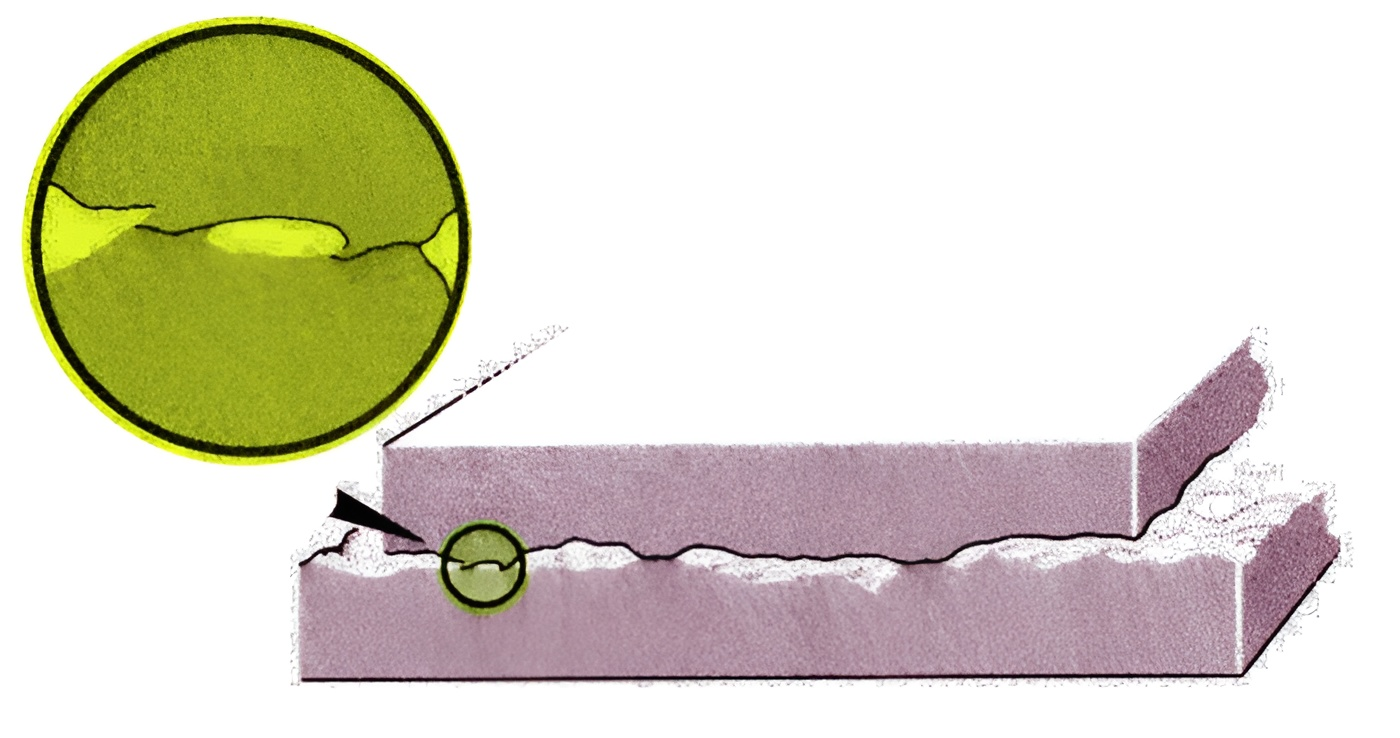
\includegraphics[width=0.45\textwidth]{images/attrito}
    \caption{asperità dei materiali}
\end{figure}\acc
L'attrito si presenta sotto due aspetti\begin{itemize}
    \item \textbf{attrito statico} : Forza esercitata su un corpo fermo su una superficie, che subisce una forza 
    \item \textbf{attrito dinamico} : Forza esercitata su un corpo in movimento che si sposta strisciando su una superficie
\end{itemize}
La modellizzazione dell'attrito prevede tale suddivisione, quando un corpo su una superficie subisce 
una forza $\bar F$, è anche soggetto ad una forza di attrito statico $\bar F_s$, essa si oppone alla prima, 
de facto è uguale in intensità e direzione, ma il verso è contrario. Se la forza applicata varia, l'attrito 
varierà con essa.\acc 
In una situazione reale però, quando si spinge un oggetto, aumentando l'intensità il corpo inizierà a muoversi, 
esiste quindi una forza di soglia sotto il quale l'attrito statico vale, una volta raggiunta tale soglia, 
il corpo si muoverà, e sarà soggetto ad attrito dinamico. In generale, tale soglia è descritta da 
$$ F_s\le \mu_s\cdot R_n$$
Dove $R_n$ è il modulo della reazione normale che subisce il corpo che poggia sulla superficie, e 
$\mu_s$ è il \textit{coefficente di attrito statico}, e dipende dal materiale dei corpi. Essendo tale attrito 
proporzionale alla reazione normale, risulta chiaro ora il perché gli oggetti posti su un piano inclinato necessitano
 di meno forza per essere spostati.\acc 
 Quindi $F_s$ è sempre uguale alla forza applicata sul corpo ma contraria di verso finché il suo modulo è minore 
 di $\mu_s\cdot R_n$. Se tale modulo è maggiore, allora il corpo sarà soggetto ad un 
 attrito dinamico $\bar F_d$
 $$ \bar F_d = -\mu_d\cdot R_n\cdot \bar \tau$$
$\mu_d$ è il coefficiete di attrito dinamico, tipicamente, per uno stesso materiale $\mu_s>\mu_d$. $\tau$ è il 
versore parallelo alla velocità del corpo che subisce tale attrito. La decelerazione che subirà 
il corpo che si muove su una superficie sarà
$$ m\bar a = -\mu_dR_n\bar \tau\implies m\bar a = -\mu_dmg\bar \tau \implies |\bar a| = -\mu_d g$$
Nella formula, si è sostituito $R_n$ ad $mg$, in quanto il modulo di tali forze è lo stesso, come già visto 
$$ R_n-mg=0$$
\begin{center}
    \includegraphics[width=0.5\textwidth]{images/attritoDinamico.eps}
\end{center}
Si noti come la decelerazione subita non dipende dalla massa del corpo, ma esclusivamente dalla reazione 
normale e dalla costante di attrito dinamico. Si ricavano le leggi della velocità e dello spostamento (nel caso 
unidimensionale) 
$$ v=v_0-\mu_dgt$$ 
$$ x=v_0t-\frac{1}{2}\mu_dgt^2$$
Il corpo si fermerà nell'istante $t_1$ in cui $v(t_1)=0$
$$ v(t_1)=0\implies v_0-\mu_dgt_1=0\implies t_1=\frac{v_0}{\mu_dg}$$
E lo spazio percorso sarà 
$$ x(t_1)=v_0t_1--\frac{1}{2}\mu_dg{t_1}^2=
v_0(\frac{v_0}{\mu_dg})-\frac{1}{2}\mu_dg{(\frac{v_0}{\mu_dg})}^2=\frac{v_0^2}{2\mu_dg}
$$
\subsubsection{Misuratore di Attrito}
Il seguento esempio, mostra com'è possibile sfruttare un piano inclinato, la cui inclinazione 
$\alpha$ è variabile, per misurare la costante di attrito statico e dinamico di un corpo. Supponiamo quindi, di posare un 
corpo su tale piano, la cui inclinazione iniziale è nulla. Cominciando a sollevare il piano (variando $\alpha$), il corpo 
rimarrà in uno stato di quiete, finché non avrà forza a sufficienza da superare l'attrito statico. Tale 
soglia equivale a $$mg\sin\alpha $$
L'attrito statico è limitato da tale valore, sia $\alpha_1$ il massimo valore dell'angolo per cui 
il corpo non si muove, in tal caso si ha 
$$ mg\sin\alpha_1=\mu_smg\cos\alpha_1\implies\mu_s=\tan\alpha_1$$
Si consideri adesso l'insieme dei valori $\alpha>\alpha_1$, per cui il corpo si muove ed è soggetto 
ad attrito dinamico. In particolare la sua forza sarà 
$$ma=m\sin\alpha-\mu_dR_n $$
Si varia l'angolo $\alpha$ per trovare il punto in cui il corpo non subisce più accelerazione, ossia $a=0$. Sia 
$\alpha_2$ tale valore 
$$ mg\sin\alpha_2-\mu_dR_n=0$$
Si ricordi $R_n=mg\cos\alpha_2$
$$ mg\sin\alpha_2=\mu_dmg\cos\alpha_2\implies \mu_d=\tan\alpha_2$$
\flowerLine 
\section{Impulso e Lavoro}
Si è visto come la dinamica permette di descrivere le equazioni 
del moto tramite le forze, in certi casi, non è chiara l'evoluzione 
nel tempo di una determinata forza, ma è comunque possibile 
avere informazioni globali sul suo comportamento grazie ad un
 integrazione. Si consideri l'integrazione della forza nel tempo in un dato 
 intervallo $[t_1,t_2]$
 $$ \int_{t_1}^{t_2}\bar F dt$$
 Le dimensioni sono espresse in $mv$, massa per velocità. Precisamente 
\begin{eqnarray}
    \int_{t_1}^{t_2}\bar Fdt =\\ 
    \int_{t_1}^{t_2} = m\dfrac{d\bar v}{dt}dt =\\ 
    m\int_{ \bar v_1}^{ \bar v_2}d\bar v = m\bar v_2-m\bar v_1=\\
    m(\bar \bar v_2-\bar v_1)
\end{eqnarray}
Risulta essere la variazione della quantità di moto, tale grandezza 
è nota come \textbf{impulso}
\eqImportante{$I=\Delta\bar p$}
Se la forza non è nota analiticamente, è possibile 
considerare la \textit{forza media} come il rapporto fra l'impulso 
e la variazione nel tempo, sia $t_2=t_1+\Delta t$
$$ \frac{I}{\Delta t}=\frac{\Delta \bar p}{\Delta t}
=\frac{1}{\Delta t}\int_{t_1}^{t_2}\bar F dt$$
Risulta utile nella descrizione dei fenomeni che agiscono in 
un breve lasso di tempo con una certa intensità, come gli urti, dette 
forze impulsive.\acc 
\redText{esempio chiodo}\acc
Quindi l'impulso deriva dall'integrazione della forza rispetto al 
tempo, essa può essere derivata anche rispetto allo spazio.
Supponiamo che vi siano una curva che unisce i punti $A$ e $B$, 
definiamo \textbf{lavoro} l'integrale 
$$ L=\int_A^B\bar Fd\bar s$$
Dove $d\bar s$ rappresenta lo spostamento infinitesimo lungo la curva, e 
$\bar Fd\bar s$ è il prodotto scalare, di cui 
$$ |\bar Fd\bar s|=Fds\cos\theta$$\begin{center}
    \includegraphics[width=0.4\textwidth]{images/lavoro.eps}
\end{center}
Le dimensioni del lavoro sono $ml^2t^{-2}$, l'unità di misura 
è il \textit{joule} e si denota $J$. Il lavoro può 
essere descritto come segue (si assuma che la massa della forza 
sia costante) 
\begin{eqnarray}
    L=\int_A^B\frac{dm\bar v}{dt}d\bar s = \\ 
    \int_A^Bmd\bar v\frac{d\bar s}{dt}
\end{eqnarray}
essendo $\frac{d\bar s}{dt}=\bar v$
\begin{eqnarray}
    \int_A^Bm\bar vd\bar v
\end{eqnarray}
Tralasciando momentaneamente l'espressione del lavoro, si noti come 
\begin{eqnarray}
    \bar v \cdot \bar v =  v^2 \text{ differenziando}\\ 
    \bar vd\bar v+\bar d\bar v\bar v=d v^2 \implies \\ 
    2d\bar v \cdot \bar v =d\bar v \bar v = \frac{1}{2}dv^2
\end{eqnarray}
quindi, tornando al lavoro
$$
    \int_A^Bm\bar vd\bar v=\int_{v_1^2}^{v_2^2}dv^2
$$
Dove $v_1$ e $v_2$ sono le velocità, rispettivamente, in $A$ ed 
in $B$ (velocità iniziale e velocità finale)$$ 
\int_{v_1^2}^{v_2^2}dv^2=\frac{1}{2}mv_2^2-\frac{1}{2}mv_1^2
$$
Definiamo $T=\frac{1}{2}mv^2$ \textbf{energia cinetica}, quindi 
$$ L=\Delta T$$
Il lavoro è \textit{la variazione dell'energia cinetica}.
\subsection{Forze Conservative}
Vediamo ora una particolare classe di forze, ossia quelle 
\textit{conservative}.\acc 
\defi{} Una forza è detta \textbf{conservativa} se il lavoro 
valutato su una curva fra due punti $A$ e $B$ è indipendente dal 
percorso considerato. Siano $\delta_1$ e $\delta_2$ due curve 
differenti, che però hanno entrambe $A$ e $B$ come punti di 
congiunzione, $\bar F$ è conservativa se 
$$ \int_{\delta_1}\bar Fd\bar s=\int_{\delta_2}\bar Fd\bar s$$
Un esempio di forza conservativa è la forza di gravità
 $\bar F_g=m\bar g$, che riscreveremo $-mg\hat y$
 $$ L=\int_{A}^B -mg\hat y d\bar s = -mg\int_A^B \hat y d \bar s$$
Si consideri il termine $\hat y d\bar s$, il modulo di $d\bar s$ 
è infinitesimo, mentre il modulo di $\hat y$ è 1. Il loro prodotto 
scalare non è altro che lo spostamento infinitesimo lungo l'asse $y$
$$
-mg\int_A^B \hat y d \bar s = -mg\int_{y(A)}^{y(B)}dy
$$
Definiamo $y(A)$ come la coordinata $y$ del punto $A$,
analogo per $y(B)$.\begin{center}
    \includegraphics[width=0.4\textwidth]{images/gravitaConservativa.eps}
\end{center}
$$ -mg\int_{y(A)}^{y(B)}dy=mgy(A)-mgy(B)$$
Definiamo $mgy=U(y)$ \textbf{energia potenziale}
$$ L=-mg\int_{y(A)}^{y(B)}dy=U(A)-U(B)=-\Delta U$$
L'energia potenziale $U$ è definita anche per le altre forze, non esclusivamente 
per la forza di gravità, che in tal caso è servita come esempio. La gravità 
è una forza \textit{uniforme}\begin{quote}
    tutte le forze uniformi sono conservative
\end{quote}
\end{document}